%----------------------------------------------------------
%	PACKAGES AND THEMES
%----------------------------------------------------------
\documentclass[aspectratio=169,xcolor=dvipsnames,handout]{beamer}

\usetheme{Darmstadt}
\usecolortheme{seahorse}
\usepackage[hangul]{kotex}
\usepackage{hyperref}
\usepackage{graphicx, array, adjustbox}
\usepackage{booktabs, multicol, multirow}
\setbeamercovered{transparent}

%------------------------------------------------------------------------------
%	MY COMMAND
%------------------------------------------------------------------------------

\newcommand{\R}{\mathbb{R}}
\newcommand{\y}{\mathbf{y}}

%------------------------------------------------------------------------------
%	TITLE PAGE
%------------------------------------------------------------------------------

\title[]{분배적 정의} % The short title appears at the bottom of every slide, the full title is only on the title page
\subtitle{노사관계의 이론과 실제}
\author[]{오성재}
\institute[CNU] % Your institution as it will appear on the bottom of every slide, may be shorthand to save space
{%
    충남대학교 경제학과\\
}
\date{\today} 

%------------------------------------------------------------------------------
%	PRESENTATION SLIDES
%------------------------------------------------------------------------------

\begin{document}

\begin{frame}
    \titlepage%
\end{frame}

\begin{frame}{목차}
    \tableofcontents
\end{frame}

\section{분배적 정의의 원칙들}
\begin{frame}[<+->]
\frametitle{분배적 정의의 원칙}
    \begin{itemize}
        \item 평등 (equalit)의 원칙
        \item 충분성 (sufficiency)의 원칙
        \item 우선 (proority)의 원칙
        \item 효용 (utility)의 원칙
        \item 공로 (merit)의 원칙
        \item 자유 (liberty)의 원칙
    \end{itemize}
\end{frame}

\begin{frame}[<+->]
\frametitle{평등의 원칙}
    \begin{itemize}
        \item 불평등은 그 자체로 정의롭지 않다. 따라서 평등 분배는 어떤 불평등 분배보다 정의롭다.
        \item 평등분배를 위해서 타인을 끌어내리는 것 역시 정당화 할 수 있다.
    \end{itemize}
    \begin{alertblock}{평등지상주의?}
    \begin{itemize}
        \item 맹인 한 사람이 존재하는 사회가 평등주의를 달성하려면?
        \item 능력이나 노력에 관계없이 모두가 동등한 결과를 얻는 사회는 정의로운가?
    \end{itemize}
    \end{alertblock}
\end{frame}

\begin{frame}[<+->]
\frametitle{충분성의 원칙}
    \begin{itemize}
        \item 모두가 충분하게 가지는 것이 중요하다.
        \item 소유의 상대적 비교 (격차의 유무, 크기)는 중요하지 않다.
    \end{itemize}
    \begin{alertblock}{빈곤의 판단}
    \begin{itemize}
        \item 상대적 빈곤: 중위소득자의 50\%.
        \item 절대적 빈곤: 일일 소득 6,000원.
    \end{itemize}
    \end{alertblock}
\end{frame}

\begin{frame}[<+->]
\frametitle{우선의 원칙}
    \begin{itemize}
        \item 분배에서 가장 열악한 위치에 처한 사람들이 개선되어야 한다.
    \end{itemize}
    \begin{figure}
        \centering
        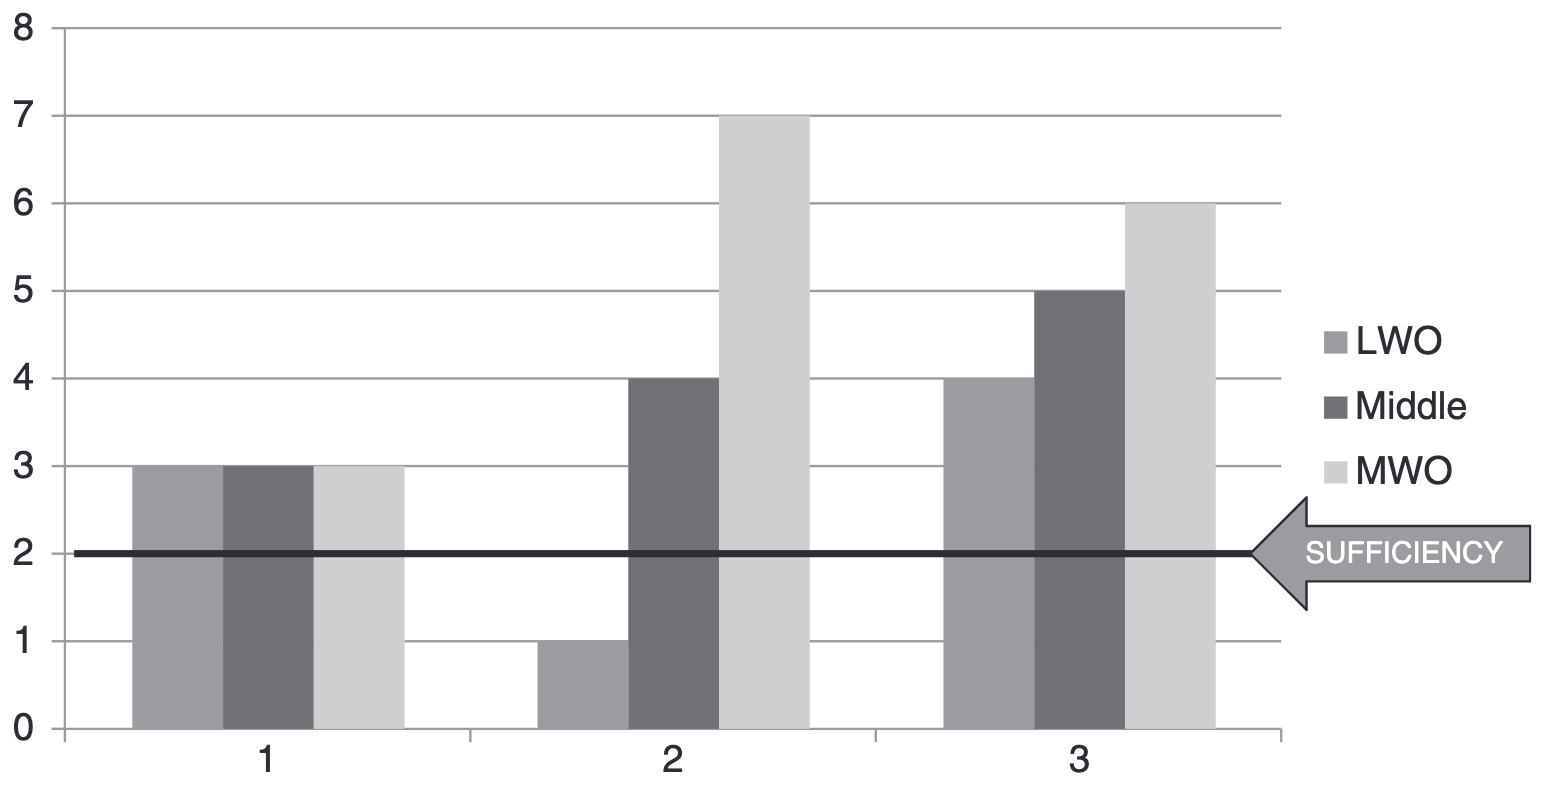
\includegraphics[width=.5\textwidth]{pic/fig1_2.png}
        \caption{간단한 소득분포}
    \end{figure}
\end{frame}

\begin{frame}[<+->]
\frametitle{효용의 원칙}
    \begin{itemize}
        \item 순효용 (이익과 손해의 차이)을 극대화 하는 분배가 정당한 분배이다.
        \item 불평등이나 빈곤의 증가는 순효용의 극대화를 위한다면 가능하다.
    \end{itemize}
    \begin{figure}
        \centering
        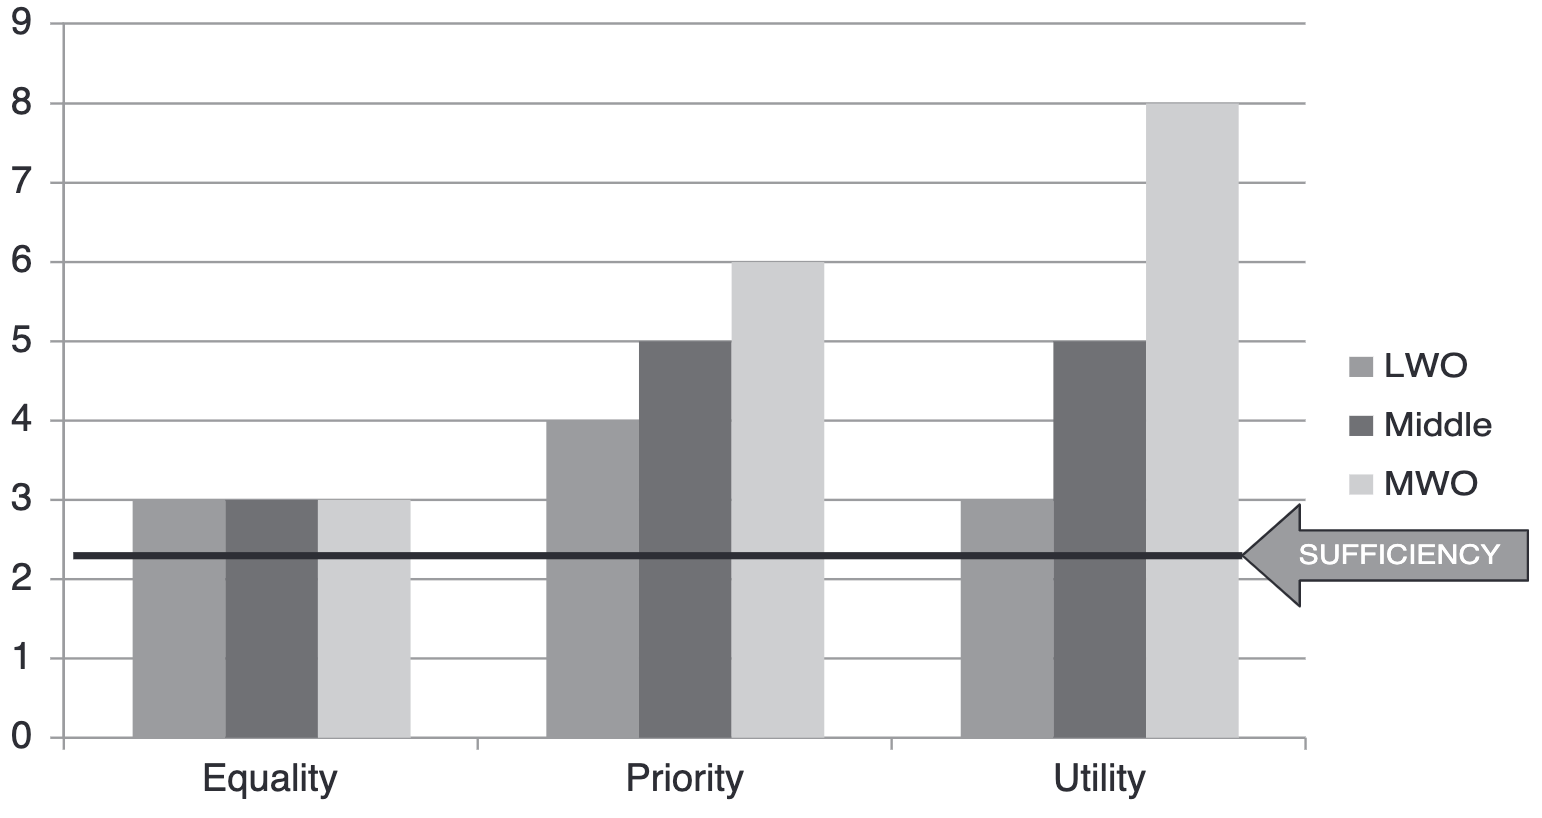
\includegraphics[width=.5\textwidth]{pic/fig1_4.png}
        \caption{분배정의 원칙에 맞는 소득분포}
    \end{figure}
\end{frame}

\begin{frame}[<+->]
\frametitle{공로의 원칙}
    \begin{itemize}
        \item 개인의 공로나 자격 (desert)을 반영한 분배가 정당하다.
        \item 자격으로서의 공로: 가장 자격있는 자가 얻는다.
        \item 노력으로서의 공로: 기여한 만큼 얻는다.
        \item 동일한 기여를 하면 같은 몫을 얻을 수 있다는 점에서 형평 (equity)의 원칙으로도 볼 수 있음.
    \end{itemize}
\end{frame}

\begin{frame}[<+->]
\frametitle{자유의 원칙}
    \begin{itemize}
        \item 정당한 분배는 사람들의 소유의 형태로 판단할 수 없다.
        \item 개인들 간에 모든 자발적 행위의 결과는 정당하다.
        \item 분배의 역사적 과정이 중요하다.
        \item 순수한 절차적 정의.
    \end{itemize}
\end{frame}

\section{우파적 자유주의}%

\begin{frame}[<+->]
\frametitle{하이에크 요약}
    \begin{itemize}
        \item 자유시장경제에 대한 유일한 대안은 계획경제.
        \item 인간의 무지 때문에 자유 시스템은 재화와 서비스를 효율적으로 생산하고 분배하는 데 계획 경제보다 우월.
        \item 상품 및 서비스의 생산 및 유통을 위한 시스템이 더 효율적일수록 평균적인 구성원이 삶의 목적을 달성하는 데 성공할 가능성이 높아짐. 
        \item 효용과 자유의 원칙은 함께 가야.
    \end{itemize}
\end{frame}

\begin{frame}[<+->]
\frametitle{하이에크의 분배정의 원칙}
    \begin{itemize}
        \item 효용의 원칙: 정의로운 사회 (그리고 정의로운 법과 제도)는 사회의 목적 (효용과 자유)을 가장 잘 촉진하는 사회.
        \item 자유의 원칙: 정당한 자원의 분배는 자유 시장에서의 자발적인 거래의 결과인 분배.
        \item 충분주의 원칙: 사회가 극도의 빈곤을 허용해서는 안되며 모든 사회 구성원이 최소한의 기본 소득을 보장함으로써 만족할 수 있는 최소한의 품위 있는 삶을 영위할 수 있도록 보장해야.
    \end{itemize}
\end{frame}

\begin{frame}[<+->]
\frametitle{법치주의 (Rule of Law)}
    \begin{itemize}
        \item 법은 구성원의 자유, 평화, 안전, 번영을 위해 필요.
        \item 법치주의의 요건을 충족하는 법만이 그 법을 따르는 구성원들의 자유와 양립.
        \item 법과 명령은 원천, 대상, 방법 세 가지에서 구분.
        \begin{itemize}
            \item 법은 적절한 입법기관에 의해 제정.
            \item 법은 특정한 사인이 아닌 전체 구성원을 동등하게 구속 (bind)함.
            \item 법은 특정인에게 특정 행동을 지시하지 않음; 단순히 행위자의 결정에 고려해야 할 추가 정보를 제공.
        \end{itemize}
    \end{itemize}
\end{frame}

\begin{frame}[<+->]
\frametitle{하이에크와 평등원칙}
    \begin{itemize}
        \item 법 앞에의 평등: 법이 특권이나 차별을 조장해선 안된다. 
        \item 최소주의적 기회의 평등:
        \begin{itemize}
            \item  자연적 운은 자유의 원칙에 위배되지 않음.
            \item  상이한 자연적 운은 경제성장의 주요한 요인.
            \item  자연적 운의 영향을 최소화 하려는 시도는 정부의 미시적 조정을 수반함.
        \end{itemize}
    \end{itemize}
\end{frame}

\begin{frame}[<+->]
\frametitle{하이에크와 공로원칙}
    \begin{itemize}
        \item 공로에 따른 분배는 옳지만, 문제는 공로의 측정방식. 
        \item 시장기구의 분배는 공로가 아닌 (시장)가치.
        \begin{itemize}
            \item 주연배우 vs. 조연배우. 
            \item 게으른 천재 vs. 성실한 범재.
        \end{itemize}
        \item  공로를 측정할 수 있다고 가정하더라도, 공로에 의한 분배는 효용의 원칙을 훼손.
    \end{itemize}
\end{frame}

\begin{frame}[<+->]
\frametitle{하이에크에 대한 비판}
    \begin{itemize}
        \item 효용의 원칙과 자유의 원칙은 조화롭기만 한가?
        \begin{itemize}
            \item 미래지향적 vs. 과거지향적 
            \item 결과중심 vs. 과정중심
        \end{itemize}
        \item 효율적이나 극단적인 불평등 사회에서 평균적인 구성원들의 미래는 과연 긍정적인가?
        \item 자유로운 시장과 법치주의만이 생산력을 극대화 하나?
        \begin{itemize}
            \item 남북한 격차.
            \item 유럽의 수정자본주의, 복지국가.
        \end{itemize}
    \end{itemize}
\end{frame}

\section{좌파적 자유주의}%

\begin{frame}[<+->]
\frametitle{공리주의 (utilitarianism)에 대한 롤즈의 비판}
    \begin{itemize}
        \item \textbf{사회}를 단순히 효용 (의 구성 요소)의 생산활동을 위한 공동체로 간주.
        \item 사회 구성원인 \textbf{개인}을 일차적으로 효용의 수단으로 간주.
        \item 효용의 총합에만 초점을 맞추므로 자원, 기회, 부담 및 권리가 \textbf{어떻게} 분배되어야 하는지에 대한 설명 부족.
        \item 개인의 효용 추구에서 어떤 \textbf{기본권}이 중요한 데 공리주의는 이를 파악하지 못하고, 따라서 그 기본권을 모두에게 동등하게 보호하지 못함.
    \end{itemize}
\end{frame}
 
\begin{frame}[<+->]
\frametitle{롤즈 vs. 하이에크}
    \begin{itemize}
        \item 롤즈와 하이에크는 분배적 정의의 원칙과 이를 실현할 사회체제의 관계가 서로 상반됨.
        \begin{itemize}
            \item  롤즈는 민주사회가 정의로운 사회이고 이를 이루기 위해 분배적 정의의 원칙을 제시. 
            \item  하이에크는 정의로운 분배를 달성하기 위한 수단으로 자유시장주의와 법치주의가 필요하다는 입장. 
        \end{itemize}
    \end{itemize}
\end{frame}

\begin{frame}[<+->]
\frametitle{원초적 입장 (original position)}
    \begin{itemize}
        \item 정의에 대한 여러 후보개념 가운데 형식적 제약을 가장 잘 만족하는 개념을 정하는 방법은?
        \item 원초적 입장은 정의의 개념을 확정하기 위한 사고 실험. 우리가 이미 가지고 있는 자료를 사용하여 그들이 의미하는 바를 명확히 하는 방법을 구성하는 것.
        \item 사회의 모든 구성원의 대표가 함께 모여 그들이 대표하는 사람들이 따라갈 정의의 개념을 선택한다고 가정.
        \item 정당에는 후보 개념 목록이 제공되며, 이 목록은 확정된 순서에 도달할 때까지 후보를 쌍으로 비교하여 순위를 정함.
    \end{itemize}
\end{frame}

\begin{frame}
\frametitle{무지의 장막 (veil of ignorance)}
    \begin{itemize}
        \item 각 대표자는 무지의 장막 뒤에 존재; 각 정당이 불편부당성을 충족하고 자신이 대표하는 정당의 의 편파적 이익을 추구하는 것을 방지.
        \begin{itemize}
            \item 대표자 본인이 누구를 대표하는지, 즉 성별, 인종, 기술, 부 또는 이와 유사한 사실에 대한 지식으로부터 무지해짐.
        \end{itemize}
        \item 무지의 장막은 불공정한 사회적 협력 조건을 제안하도록 유도할 수 있는 지식으로부터 당사자를 배제하지만, 정의에 대한 후보 개념의 순위를 매기기에는 충분한 지식을 제공.
        \item 따라서 당사자는 자신이 대표하는 사람들이 선에 대한 개념을 갖고 있다는 것만을 알고 자신의 상황에 대한 일반적인 사실을 알고 있음.
    \end{itemize}
\end{frame}

\begin{frame}[<+->]
\frametitle{기본재 (primary good)}
    \begin{enumerate}
            \item  기본권과 자유.
            \item  이동의 자유와 직업 선택의 자유.
            \item  직위와 직책에 접근할 수 있는 권한, 특권 및 기회.
            \item  소득과 재산.
            \item  자존감의 사회적 기반.
    \end{enumerate}
\end{frame}

\begin{frame}[<+->]
\frametitle{정의의 원칙}
    \begin{enumerate}
        \item  1.동등한 기본권의 원칙: 모든 사람은 최대한의 평등한 기본 자유를 누릴 권리가 있으며, 이는 다른 사람들의 동일한 자유와 양립할 수 있어야 한다.
        \item  2.민주적 평등의 원칙: 
        \begin{itemize}
            \item  a. 공정한 기회 균등 원칙: 사회적, 경제적 불평등은 모든 사람에게 공정한 기회가 제공되는 조건에서만 허용된다. 즉, 같은 재능과 의지력을 가진 사람은 배경과 상관없이 동등한 기회를 가져야 한다.
            \item  b. 차등의 원칙: 불평등이 허용되는 경우, 그것은 사회의 가장 불리한 위치에 있는 사람들에게 최대의 혜택을 제공하는 방식이어야 한다.
        \end{itemize}
    \end{enumerate}
\end{frame}

\begin{frame}[<+->]
\frametitle{우선의 원칙}
    \begin{itemize}
        \item 우선 원칙: 첫 번째 원칙은 두 번째 원칙에 우선. 두 번째 원칙의 a 항목이 b 항목보다 우선.
        \item 우선순위가 낮은 원칙에 대한 큰 이익을 위해 우선순위가 높은 원칙을 타협할 수 없다는 의미.
        \item 우선 순위 규칙은 권리와 자유의 제한은 물론 기회의 평등과 타협을 허용.
        \begin{itemize}
            \item 차별 철폐 정책은 어떤 면에서는 기회 평등을 침해할 수 있지만 그럼에도 불구하고 다른 면에서는 평등한 권리 또는 기회 평등을 보장하는 데 정당화될 수 있음.
        \end{itemize}
    \end{itemize}
\end{frame}

\section{자유지상주의}%

\begin{frame}[<+->]
\frametitle{자유지상주의}
    \begin{itemize}
        \item 자유지상주의는 개인의 삶에 국가에 의한 법에 강압적 지배가 없어야 한다는 사상 중 하나.
        \begin{itemize}
            \item 모든 개인은 자신의 행동이 평등한 타인의 자유권을 침해하지 않는 한, 스스로 무엇을 할 것인지 결정할 자유가 있음.
        \end{itemize}
    \item 국가는 구성원들의 활동의 자유가 서로 일관되게 하기 위해서만 간섭.
        \begin{itemize}
        \item 국가는 폭력, 절도, 기만 등으로부터 구성원을 보호하는 역할.
        \item 가부장적 정부 (예: 안전벨트 착용 의무화, 마약 사용 금지, 결혼에 대한 특정 견해 시행 등)의 역할을 하거나 재분배를 추구해서는 안됨.
        \item 그러한 국가권력 행사는 구성원 일부의 자유를 부당하게 제한하기 때문.
        \end{itemize}
    \item 이러한 자유지상주의 원칙은 단순하면서도 강력함.
    \end{itemize}
\end{frame}

\begin{frame}[<+->]
\frametitle{국가의 크기}
    \begin{itemize}
        \item 자유지상주의자들이 이야기 하는 작은 국가의 기준은 무엇인가?
        \begin{itemize}
            \item 국가의 규모는 지출 측면에서 (예: GDP대비 정부부채).
            \item 공공 고용 측면에서 (예: 총인구 대비 공무원 수).
            \item 구성원의 생활에 대한 규제의 갯수.
        \end{itemize}
        \item Nozick은 권위의 범위 측면에서 국가의 크기를 정의.
        \begin{itemize}
            \item 절대 군주는 백성의 생활 전체를 통제할 수 있는 강력한 권한을 가질 수 있지만 직위나 법을 만들지 않고도 가능 (군주의 뜻 하나로도 가능).
        \end{itemize}
    \end{itemize}
\end{frame}

\begin{frame}[<+->]
\frametitle{작은 국가}
    \begin{itemize}
        \item 가장 작은 국가는 주어진 영토에서 강제력 사용을 독점하여 다른 대리인이 강제력을 사용할 수 없도록 하는 국가 (긴급 상황 제외).
        \item 작은 국가는 주어진 영토에서 강제 사용에 대한 독점을 행사하고 영토에 거주하는 모든 개인의 권리가 보호되도록 보장하며 그밖에는 어떤것도 하지 않는 국가.
        \begin{itemize}
            \item 공공재, 빈민구제, 의료, 교육마저도 제공하지 않음. 단, 사회구성원의 (자유)권리를 보장하기 위해 필요한 경우는 예외.
            \item 구성원의 원래 권리와 획득한 권리를 확보하는 것 이외의 목표를 추구하는 국가는 작은 국가보다 ``더 큰'' 국가.
        \end{itemize}
    \end{itemize}
\end{frame}

\begin{frame}[<+->]
\frametitle{소유의 정의}
    \begin{itemize}
        \item Nozick은 정부가 구성원들에게 분배해야할 대상 그 자체가 없다고 주장.
        \item 분배는 어떤 정당한 분배로부터 합법적인 수단을 통해서 이뤄질 때만 정당.
        \item 합법적인 수단은 자원의 최초 획득 그리고 재화와 용역의 이전을 규정짓는 원칙에 의해 지정.
    \end{itemize}
\end{frame}


\begin{frame}[<+->]
\frametitle{자격 이론}
    \begin{itemize}
        \item Nozick의 분배 정의는 자격의 문제; 자격을 갖추 소유만이 정의.
        \begin{itemize}
            \item 정당한 획득의 원칙: 소유된 역사가 없는 자원의 원초적 할당에 대하여.
            \item 정당한 이전의 원칙: 재화와 용역의 개인간 교환에 대하여.
            \item 교정의 원칙: 위 두 원칙이 위반될 경우에 대하여.
        \end{itemize}
    \end{itemize}
\end{frame}
  
\begin{frame}[allowframebreaks]
\frametitle{정당한 획득의 원칙}
    \begin{itemize}
        \item 자연의 상태에는 다양한 (천연)자원이 존재.
        \item 인간의 능력 (노동력)과 결합하여 새로운 자원으로 전환.
        \item 자원의 소유에는 두 가지 조건이 존재:
        \begin{itemize}
            \item 개인은 자신이 훌륭하게 사용할 수 있는 정도 이상을 가질 수 없음.
            \item 타인을 위하여 충분하면서 훌륭한 잔여물이 존재해야.
        \end{itemize}
        \item 원초적 소유는 타인의 상황을 악화 시키지 말아야.
    \framebreak%
        \item 정당한 이전은 당사자의 자발적 선택을 알린다는 점에서 하는 자유의 원칙.
        \item 정당한 이전을 통해 물건을 얻는다면, 정당한 획득을 만족.
        \item 정당햔 이전이 반복되는 한 모든 획득은 정당함.
        \item 정당한 획득의 조건은 타인의 상황을 악화시키지 말아야 하고, 이는 정당한 이전의 원칙에 대한 제약으로 작용 (예: 물과 같은 필수재의 독점).
    \end{itemize}
\end{frame}

\begin{frame}[<+->]
\frametitle{교정의 원칙}
    \begin{itemize}
        \item 교정의 원칙은 단순하면서 강력함; 불의는 교정되어야 한다.
        \item 그렇다면 불의란 무엇인가?
        \item 모든 부당한 이전 (예: 장물은 취득도 불법).
        \item 그러나 Nozick은 부당한 이전이 어디까지 거슬러 올라가야 하는가에 대해서는 말하지 않음.
        \begin{itemize}
            \item 각국의 수탈당한 해외 문화재.
            \item 식민지 경험에 대한 보상 등등.
        \end{itemize}
    \end{itemize}
\end{frame}

\begin{frame}[allowframebreaks]
\frametitle{정의로운 분배: 자유, 소유권, 계약}
    \begin{itemize}
        \item Nozick은 소유에 대한 개인의 권리라는 관점에서 분배적 정의를 설명.
        \item 정당한 획득 또는 정당한 이전을 통한 획득만이 소유권을 인정받음.
        \item 이 과정을 통한 소유가 아닌 경우, 교정의 원칙이 작동하여 현재의 소유를 부당하게 하는 모든 불의의 교정을 강제.
        \item 교정의 원칙이 충족되고 과거에 교정이 필요한 부당함이 현재 소유로 이어지지 않으면 현재 소유는 정당하며, 모든 개인은 자신이 소유를 인정받을 자격을 획득.
    \framebreak%
        \item 하나의 분배가 다른 분배상태에서 이전에 의한 결과라면, 어떤 여건에 관계없이 그 자체로 정당.
        \item 빈곤 또는 불평등의 정도, 개인의 특성이나 운, 행복감 등등의 어떤 요소도 무관.
        \item 자원의 분배가 정당성은 소유자의 자격을 통해서만 판단.
        \item 분배의 정의는 분배의 역사의 결과이며, 그 역사가 정의롭다면 분배도 정의로움.
    \end{itemize}
\end{frame}


\end{document}
